\setlength{\parskip}{12pt}
\setlength{\parindent}{0cm}
\renewcommand{\arraystretch}{1.2}
\setcounter{secnumdepth}{4}

\geometry{top=2.5cm, bottom=2.5cm, left=2.5cm, right=2.5cm}
\begin{document}



\renewcommand{\listtablename}{Índice de tablas}
\renewcommand{\tablename}{Tabla}

\definecolor{light-gray}{gray}{0.87}  

\begin{titlepage}
\hspace*{-3.5cm}
    \begin{minipage}{\textwidth}
        \vspace{-2.5cm}
        \begin{center}
    

            
\includegraphics[width=\paperwidth]{graphics/LogoEHU.PNG}
        \end{center}
    \end{minipage}

\vspace{1cm}

\hspace{-3.1cm}
\noindent\fcolorbox {light-gray}{white}{

    \parbox{\paperwidth}{
     \begin{center}
     \large Gradu amaierako lana /Trabajo fin de grado
    \\
             \large Ingenieritza Kimiko gradua/ Grado en Ingeniería Química

\end{center}
    }
    }


\vspace{0.8cm}

\noindent\hspace*{-2.5cm}%
\colorbox{light-gray}{\begin{minipage}{\paperwidth}%

    \vspace{1cm}

    \color{RoyalBlue}
    \centering\Large\textbf{ Lanaren izenrua / Título del trabajo}
    \\
    \centering\textmd{ Lanaren azpitituloa / Subtitulo del trabajo}


    \vspace{6cm}\mbox{}
  \end{minipage}
}

\begin{flushright}
 Egilea/ Autor/a:
\\
Andoitz Campo Pérez
\\
Zuzendariak/Directores/as:
\\
Asier Aranzabal Maiztegi
\\
XXX XXX                      
\\
\end{flushright}

\begin{center}
\noindent\fcolorbox {white}{white}{

    \parbox{11cm}{
         \begin{center}
    \footnotesize © 2021, se puede proteger poniendo nombre y apellido/izen abizenak ezarriz babes zaitezke edo lizentzia CC batekin babestu / o con una licencia CC
    \\
   \small http://es.creativecommons.org/blog/licencias/

        \end{center}
    }
    }
\end{center}

\hspace{-3.2cm}
\noindent\fcolorbox {light-gray}{white}{
    \begin{minipage}[]{1000pt}

        \parbox{\paperwidth}{
            \begin{center}
    
                 Leioa, 2021eko XXXren XXa / Leioa, XX de XXX de 2021

            \end{center}
        }
    \end{minipage}
}

\end{titlepage}

\tableofcontents

\newpage 

%%%%%%%%%%%%%%%%%%%%%%%%%%%%%%%
%Hemendik aurrera hasi lana idazten%
%%%%%%%%%%%%%%%%%%%%%%%%%%%
% **************************************************************************** %
%                                                                              %
%                                                     ::::::::  :::::::::      %
%    sec_intro.tex                                      :+:      :+:    :+:    %
%                                                    +:+        +:+    +:+     %
%    By: A. Campo <andoitzcp@gmail.com>              +#+        +#++:++#+      %
%                                                    +#+        +#+            %
%    Created: 2022/11/18 22:55:54 by A. Campo        #+#    #+# #+#            %
%    Updated: 2023/02/16 04:35:39 by acampo-p         ###   ########.fr        %
%                                                                              %
% **************************************************************************** %

\section{INTRODUCCIÓN}\label{sec:intro}

El sector de la automoción,
engloba una gran variedad de industria y servicios dedicados a servirla.
Se estima que la aportación económica total de las actividades relacionadas,
en este sector, asciende a un 11\% del PIB,
lo que la convierte en la industria manufacturera que más ingresos aporta
después  del 18,8\% del PIB que posee la industria agroalimentaria española
\citep{caixabank2021analisis}.

En este sector, el vehículo de propulsión autónoma,
es generalmente utilizado tanto por los servicios de transporte a pasajero,
como por los servicios logísticos dedicados al transporte de mercancías.
Entre los componentes que forman el vehículo autónomo,
se encuentran las cubiertas o neumáticos,
los cuales se comportan como enlace entre el vehículo y el pavimento.
Este nexo permite una transmisión eficiente
de la energía producida por el motor de combustión interna,
y a su vez, sus propiedades elásticas atenúan las irregularidades de la vía.

La industria manufacturera de cubiertas,
ha mantenido un incremento sostenido en su producción en los últimos años,
como puede observarse en la Figura \ref{fig:1_global_prod_evo}.
El mercado de neumáticos es liderado por dos empresas: Bridgestone y Michelin
\citep{rodgers2020tire}.
Las demás empresas compiten entre ellas
a una magnitud inferior a los líderes del sector,
como se aprecia en la Figura \ref{fig:1_brand_revenue}.

\begin{figure}[h]
	\begin{center}
		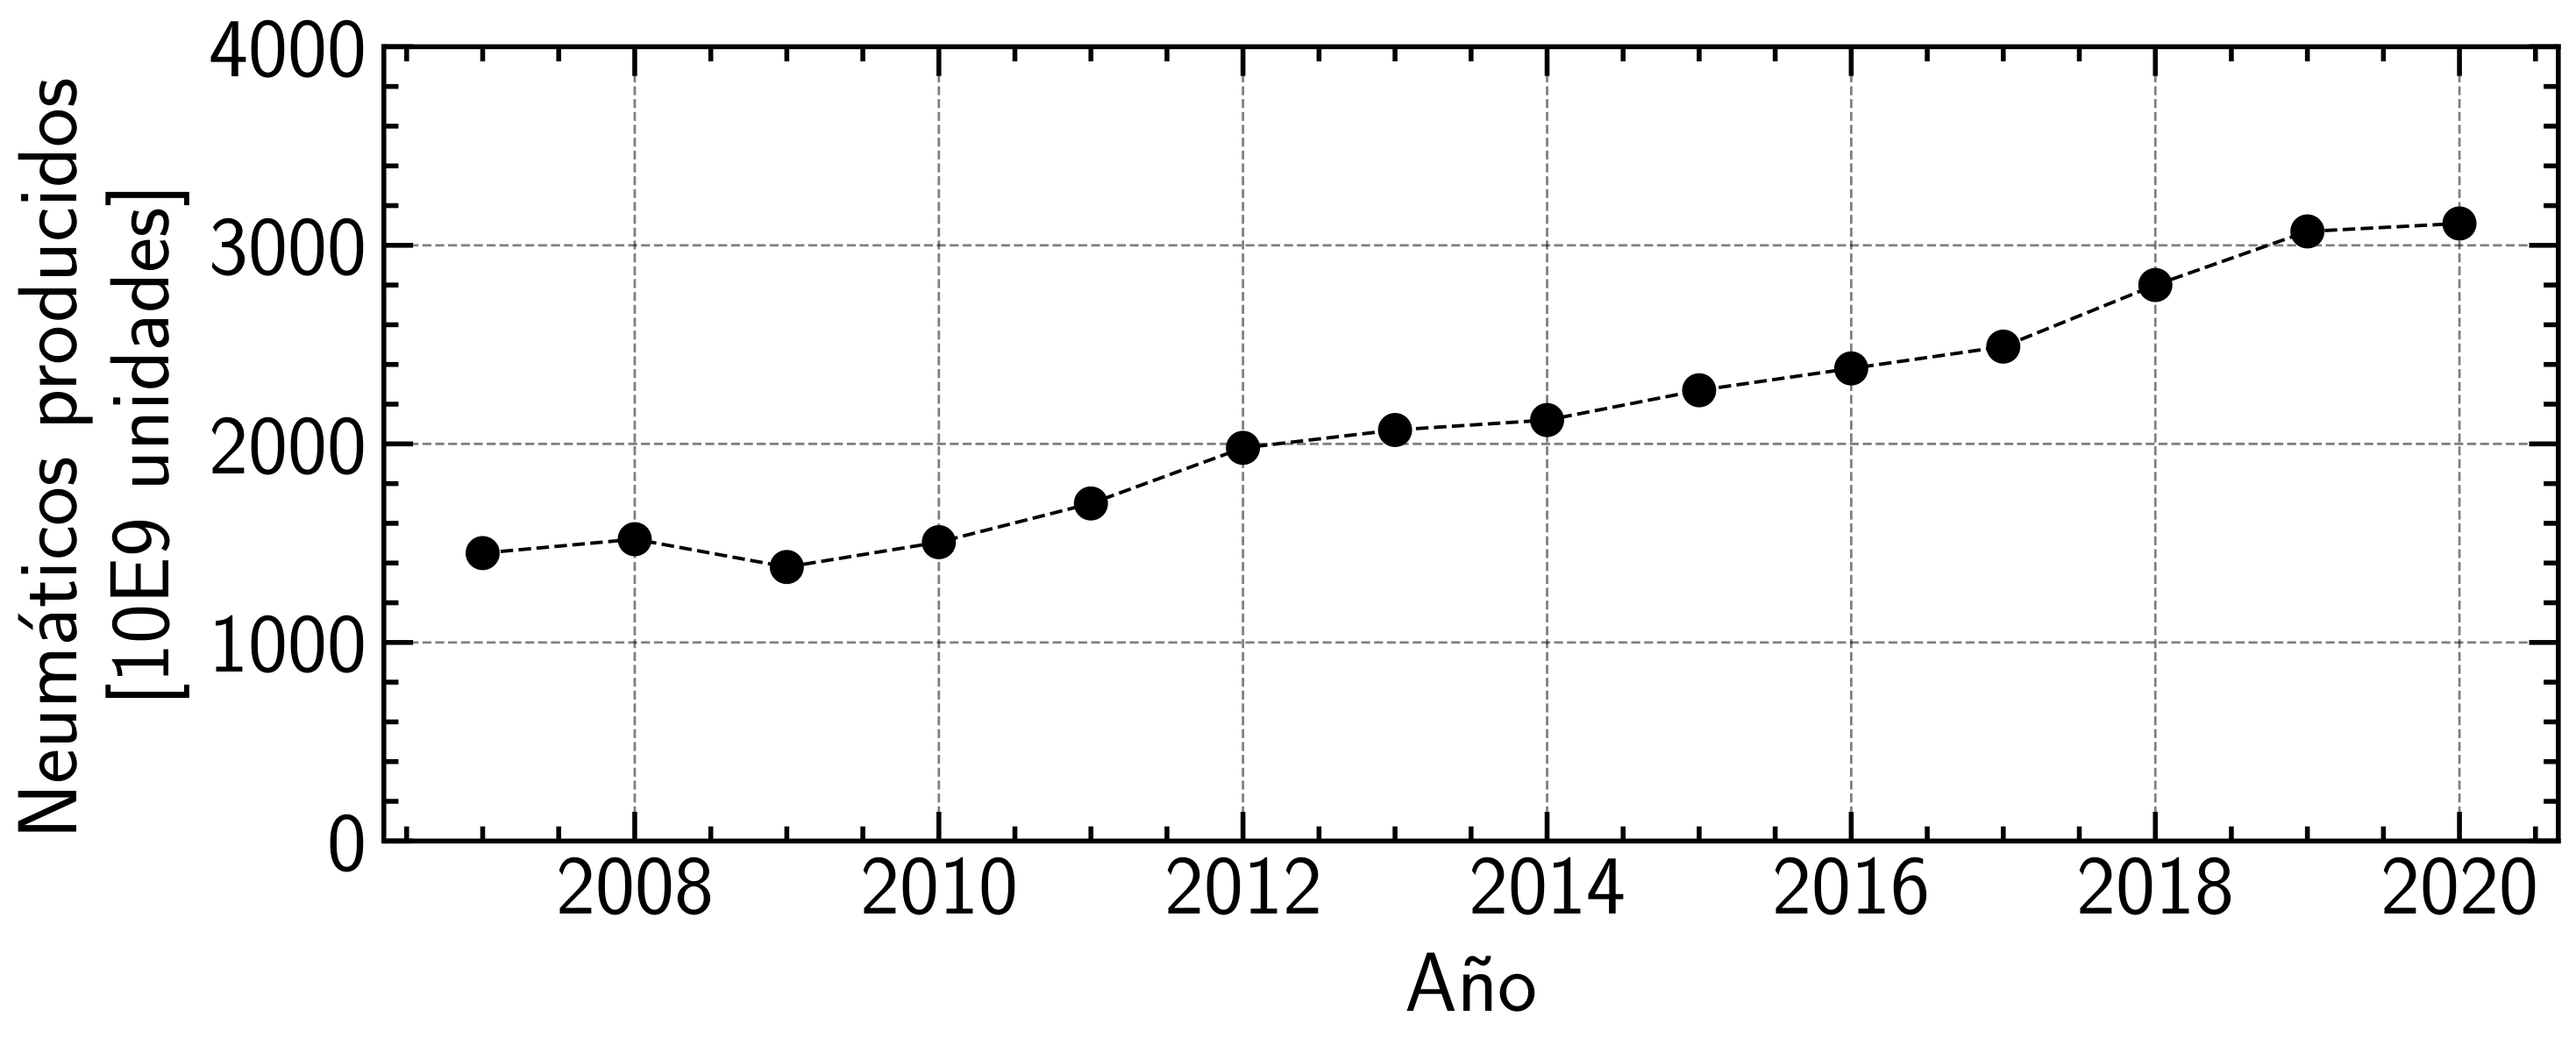
\includegraphics[width=\textwidth]{fig/1_global_prod_evo.PNG}
	\end{center}
	\caption{Evolución de la producción mundial de cubiertas \citep{rodgers2020tire}.}
	\label{fig:1_global_prod_evo}
\end{figure}

 \begin{figure}[h]
	\begin{center}
		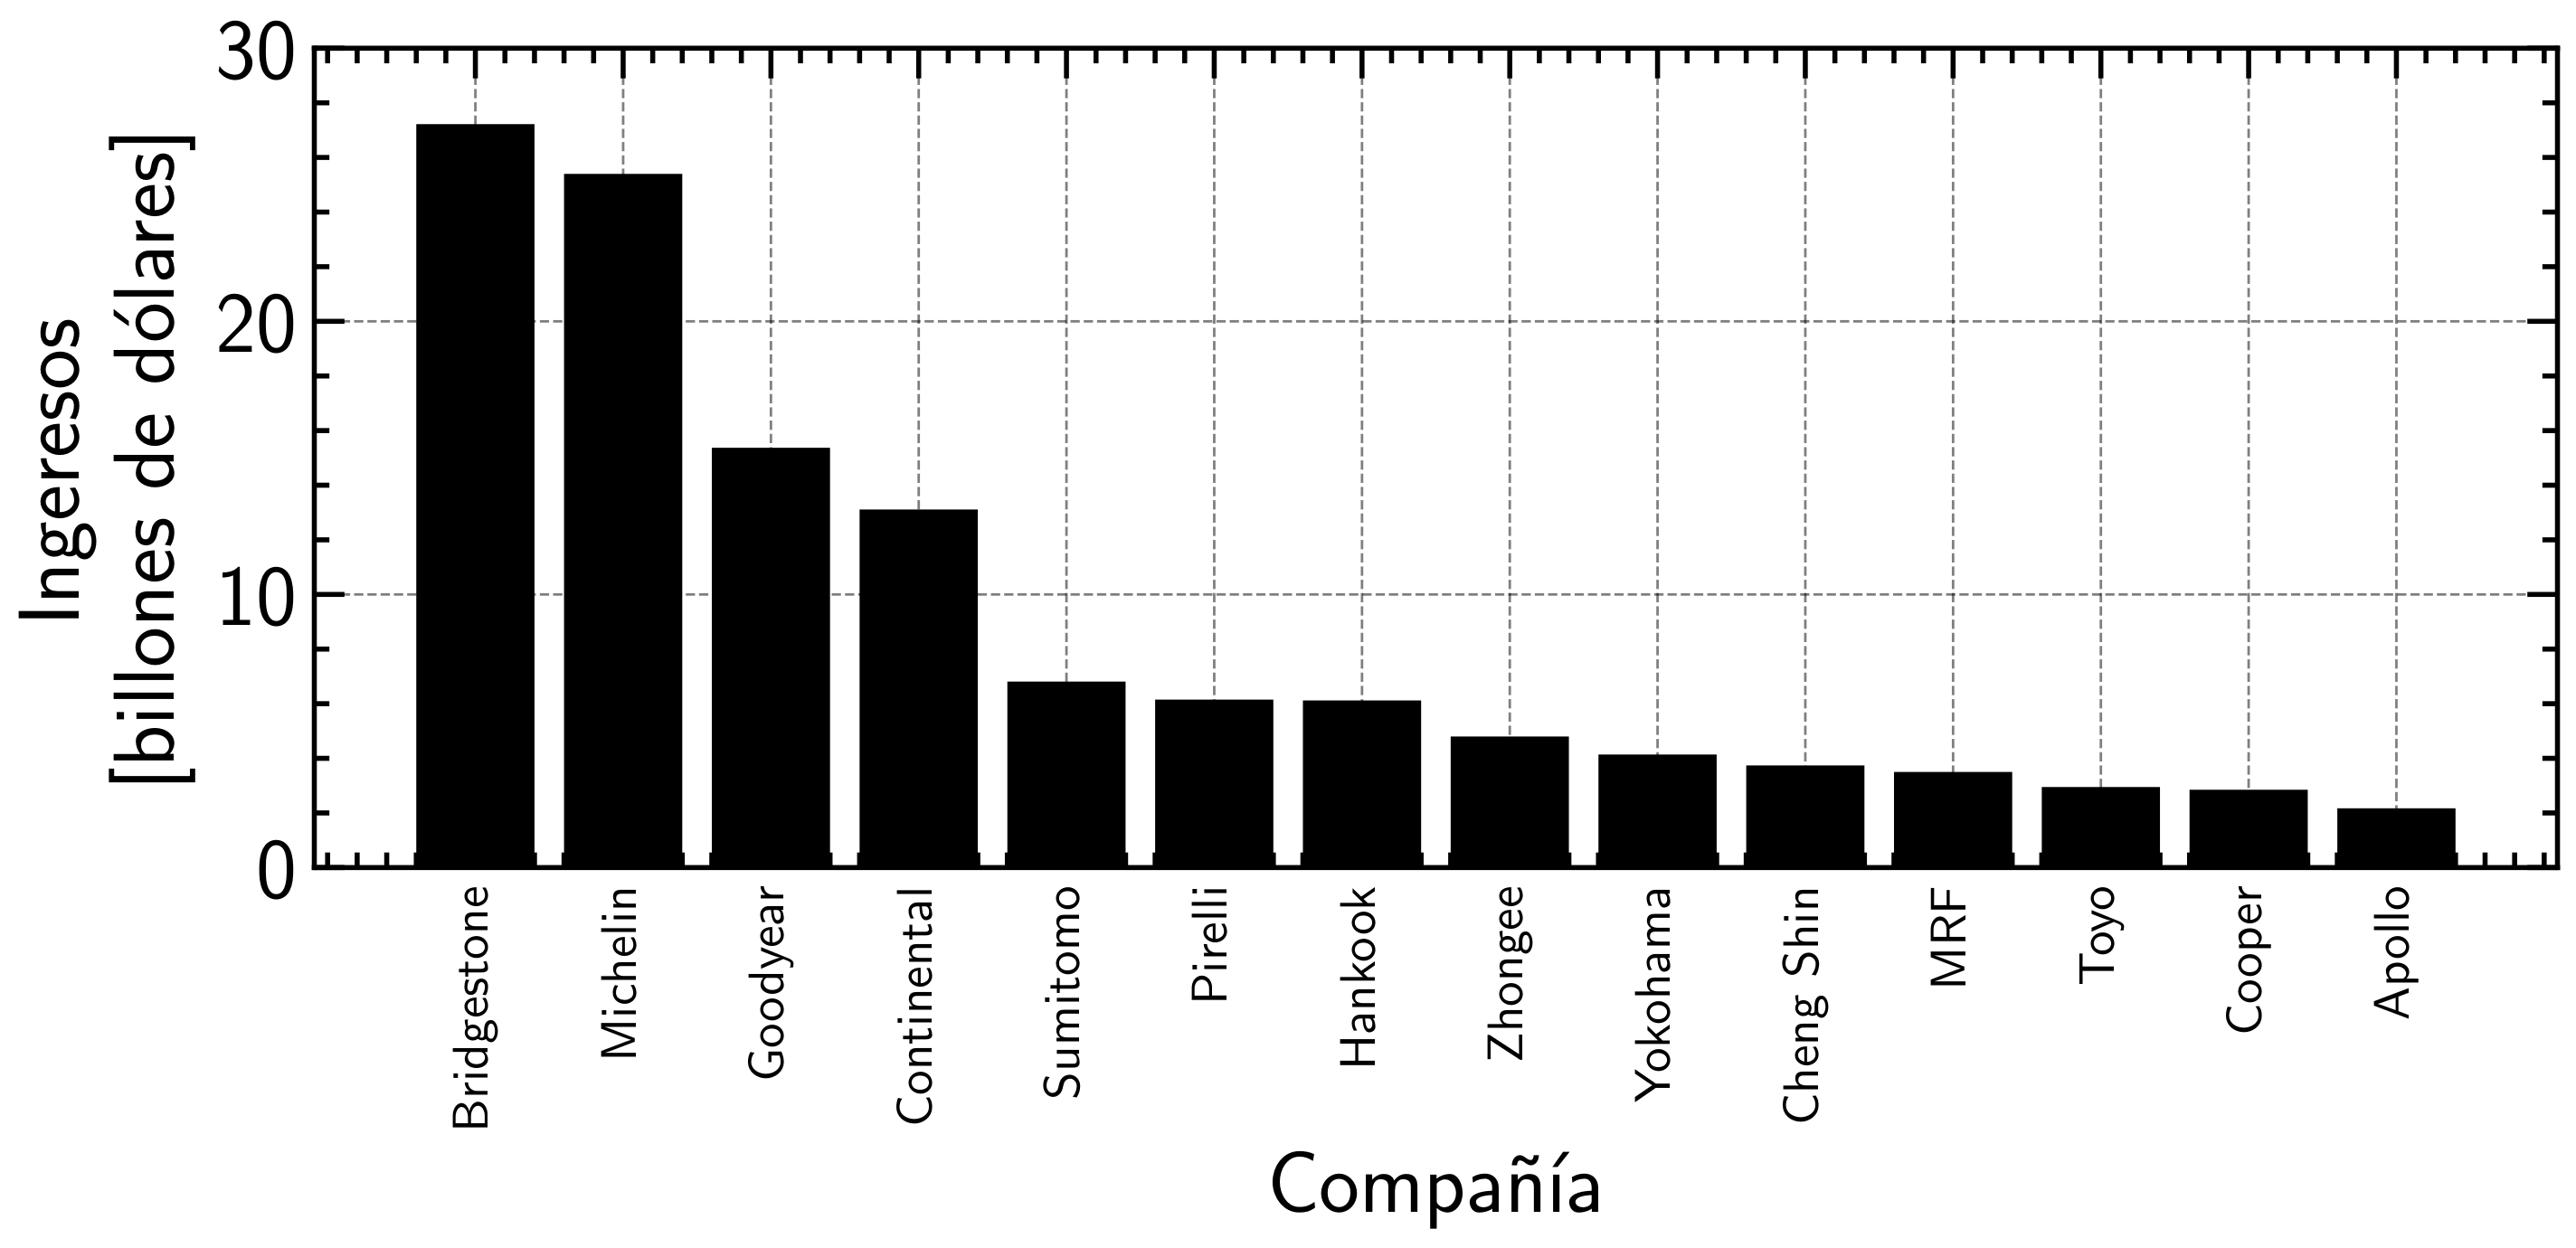
\includegraphics[width=\textwidth]{fig/1_brand.revenue.PNG}
	\end{center}
	\caption{Ingresos de los fabricantes de neumáticos más relevantes en 2019 \citep{rodgers2020tire}.}
	\label{fig:1_brand_revenue}
\end{figure}

La elevada competitividad característica del mercado,
sumada a la emergente comercialización de producto asiático,
incentiva a las establecidas multinacionales, a tomar un enfoque innovativo,
con la intención de mantener su liderazgo \citep{chicu2020current}.
El esfuerzo invertido en innovación,
por una parte, intenta alcanzar sus objetivos
mediante el rediseño y la mejora del producto.
Mientras que por la otra,
trata de optimizar sus procesos y reducir desperdicios,
mediante la automatización y el uso inteligente de los recursos disponibles.

A la hora de implementar mejoras, ya sea a un producto o a un proceso,
la monitorización de los resultados se vuelve esencial.
El producto o proceso experimental debe satisfacer las expectativas del cliente,
y a su vez, cumplimentar la legislación vigente,
como los estándares de calidad y medio ambiente.
La monitorización de estas mejoras implica un coste elevado,
a nivel temporal y económico, ya que estas deben ser puestas a prueba.
En el caso del producto, su industrialización,
supone reservar recursos que podrían ser destinados a la producción regular.
Desde la materia prima utilizada
en la elaboración de estos productos experimentales,
a través de cada máquina ocupada para transformarlo,
hasta llegar al laboratorio de calidad,
donde se realizan ensayos para otorgar feedback a la empresa.

En las empresas de neumáticos, el laboratorio de Calidad del Producto (LCP),
es el encargado de llevar a cabo los ensayos relevantes
para asegurar la conformidad de la producción.
A diario se cerciora de que los neumáticos manufacturados dentro de la planta
cumpla con los estándares de calidad definidos por la compañía.
El laboratorio logra asegurar la calidad del producto,
mediante un control estadístico de las muestras
elegidas al azar por cada gamma de producto.
Paralelamente, una fracción de los recursos disponibles,
es demandada por los proyectos de industrialización.
Obligando al departamento a equilibrar ambas necesidades.

En un entorno con recursos limitados,
donde la demanda no cesa de incrementar,
es cuestión de tiempo que los recursos se agoten
y la capacidad del laboratorio se vea sobrepasada.
Para hacer frente a esta situación,
y poder mantener el esencial ritmo
marcado por los estándares de control de calidad e industrialización,
debe realizarse un escalado de los recursos del LCP.
A fin de que la expansión, de este sistema complejo,
se desarrolle de la manera óptima,
dirigir  un estudio del impacto sobre
las posibles inversiones resulta conveniente.
Debido a que experimentar con el sistema real,
y desarrollar una solución analítica no es factible,
se ha propuesto el uso de la simulación.
Dentro de los tipos de simulación, existen varias alternativas.

\begin{itemize}
	\item Simulación Monte Carlo: Este tipo de simulaciones toma el nombre
		del famoso casino ubicado en Mónaco.
		Este tipo de simulación se caracteriza por desencadenar eventos al azar
		con el fin de obtener los resultados esperados.
		Se emplea con el fin de aproximar
		expresiones matemáticas complejas.
		\citet{owen2016monte} describen la simulación de Monte Carlo,
		como un método para aproximar integrales
		mediante muestras promedio de valores enteros.
		Este método se puede usar, por ejemplo,
		para determinar la probabilidad de que
		un dado obtenga como resultado
		al menos un 5 en 4 de cada diez tiradas.
		El método Monte Carlo es apropiado para sistemas estáticos
		\citep{lawson2008monte},
		es decir, sistemas que no tienen en cuenta el paso del tiempo. 
		
	\item Sistemas Dinámicos (SD): La metodología de los SD trata de capturar
		el comportamiento de un sistema mediante
		su representación en un diagrama de flujo
		\citep{sweetser1999comparison}.
		Esta metodología, toma un enfoque cualitativo,
		apto para gerentes de empresa y organizaciones gubernamentales.
		Los SD están adaptados para sistemas continuos,
		siendo poco prácticos en un ambiente manufacturero,
		donde interrupciones como cambios de turno,
		Reparaciones de máquina, descansos de operario \ldots suceden a menudo.

	\item Simulación de Eventos Discretos (DES):
		Las DES toman el enfoque de representar sistemas reales
		mediante la ejecución y concatenación
		de procesos en un entorno virtual.
		Esta representación computacional se asemeja al sistema real.
		La DES ha demostrado su capacidad de resolver
		problemas de optimización en sistemas estocásticos.
		Como menciona el \citet	{allen2011introduction},
		su versatilidad ha sido demostrada en numerosos ámbitos,
		como aplicaciones militares,
		sistemas sanitarios,
		problemas logísticos
		y optimización de procesos de manufacturación.
\end{itemize}

\subsection{EL LABORATORIO DE CALIDAD DEL \newline PRODUCTO}

A lo largo del proceso de fabricación de una cubierta,
son varios los estándares de calidad que debe cumplir el producto
para que pueda ser vendido en los distintos mercados a nivel global.
Desde la composición química de las materias primas usadas,
hasta las propiedades físicas del producto finalizado,
la certificación de que el producto se halla dentro de
los límites especificados, asegura un producto de calidad.

En el proceso final de control de calidad
que se lleva a cabo en un laboratorio de evaluación del producto,
estos son los ensayos principales.

\begin{itemize}
	\item Ensayos \textit{Endurance}
	\item Ensayos \textit{Rolling Resistance}
	\item Ensayos dimensionales
\end{itemize}

En un LCP,
se debe satisfacer la demanda de ensayos de los siguientes procesos:

Por una parte, los procesos de Conformidad de la Producción (CP),
encargados de aseguramiento de la calidad
del producto destinado a la venta a clientes
Por otra parte, los procesos para el desarrollo de nuevos productos,
propios de las actividades de industrialización (IND),
encargados de desarrollar nuevas líneas del producto,
y optimizar los procesos de producción
mediante cambios controlados que suceden en grupos reducidos.
Finalmente, existen encargos que
no encajan con las 2 anteriores categorías, (EXT).
Para este caso, en el LCP, se ha estimado que,
estas 3 fuentes de muestras de ensayo
suman la cantidad descrita en la Tabla~\ref{tab:2_tbl_actual_demand}.
La cual está cerca, de los límites de capacidad teóricos
para un laboratorio con el equipamiento descrito en
las Tablas~\ref{tab:3_tbl_sim_det} y~\ref{tab:3_tbl_rsrc}.
Las perspectivas de futuro, prevén un incremento continuado de la actividad,
por lo que es habitual que el LCP afronte demandas superiores a su capacidad.

\begin{table}
	\centering
	\caption{Suma de la demanda típica de ensayos en un LCP.}
	\documentclass[varwidth=\maxdimen]{standalone}
\usepackage[utf8]{inputenc}
\usepackage[spanish]{babel}
\usepackage{booktabs}

\begin{document}

\begin{tabular}{ l c }
	\toprule
	Ensayo & Demanda (unds.) \\
	\midrule
	Endurance	& 280 \\
	Rolling		& 760 \\
	Dimensional	& 140 \\
	\bottomrule
\end{tabular}

\end{document}

	\label{tab:2_tbl_actual_demand}
\end{table}

El flujo de los procesos llevados a cabo en el laboratorio,
se representa en la Figura~\ref{fig:2_fc_lep_diagram}.

\begin{figure}
	\begin{center}
		\includestandalone{fig/2_fc_lep_diagram}
	\end{center}
	\caption{Diagrama de flujo de los procesos llevados a cabo en el LCP.}
	\label{fig:2_fc_lep_diagram}
\end{figure}

\subsubsection{Ensayos \textit{Endurance}}
El ensayo \textit{Endurance} esta destinado a medir la fatiga
que pueden llegar a soportar los materiales internos de la cubierta.
Los materiales internos de una cubierta son señalados
en la Figura~\ref{fig:2_tirecs}, como \textit{Steel Belt},
los cuales son capas de hilos de acero entrecruzados que
aportan resistencia a la zona más expuesta de la cubierta.
Las altas temperaturas y cargas a las que son sometidas las cubiertas
producen una separación entre las capas de acero internas.
Esta separación crea una deformación en la superficie de la cubierta.
Cuando una deformación se detecta el ensayo concluye.
Una vez finalizado, un operario corta y pule 2 secciones,
una de ellas se toma en el origen de la separación de las capas interiores,
la restante se toma a 180º del origen de la deformación.

\begin{figure}[H]
	\begin{center}
		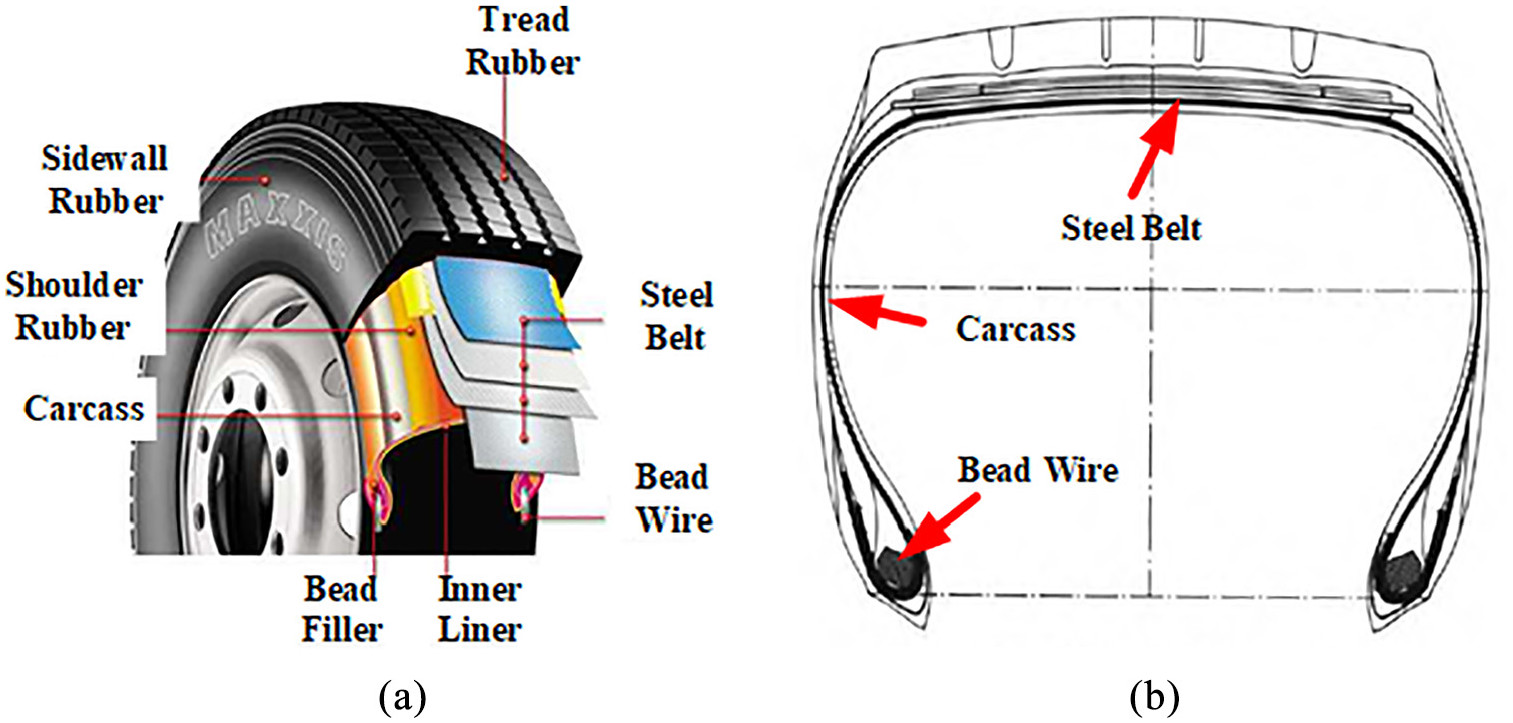
\includegraphics[width=\textwidth]{fig/2_tirecs}
	\end{center}
	\caption{Diagrama de la composición de una cubierta}
	\label{fig:2_tirecs}
\end{figure}

Los ensayos son llevados a cabo en la máquina expuesta
en la Figura~\ref{fig:2_endurance_machine}.
La máquina se encuentra en una sala aislada acondicionada a 40 º$C$.
La carga a la que son sometidas las cubiertas varía durante el ensayo
en incrementos comúnmente llamados pasos.
En la Tabla~\ref{tab:1_tbl_qced_steps} se exponen detalles de cada paso.
La carga a la que es sometida cada cubierta viene determinada
por el índice de carga (LI) grabado en el costado de la cubierta,
a su vez, la velocidad viene determinada por el fabricante.
El LI se muestra en el Anexo~\ref{apnd4}.

\begin{table}
	\centering
	\caption{Pasos de un ensayo \textit{Endurance}.}
	\documentclass[varwidth=\maxdimen]{standalone}
\usepackage[utf8]{inputenc}
\usepackage[spanish]{babel}
\usepackage{booktabs}

\begin{document}

\begin{tabular}{ l c c }
	\toprule
	Paso	& Carga (\%)	& Duración (h) \\
	\midrule
	1		& 66	& 7 \\
	2		& 82	& 16 \\
	3		& 100	& 24\\
	4-12	& +10	& 6 \\
	\bottomrule
\end{tabular}

\end{document}

	\label{tab:1_tbl_qced_steps}
\end{table}

\begin{figure}[H]
	\begin{center}
		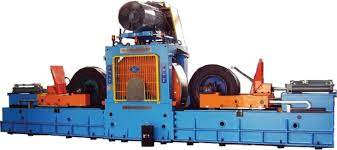
\includegraphics[width=\textwidth]{fig/2_endurance_machine}
	\end{center}
	\caption{Máquina utilizada en los ensayos \textit{Endurance}. 
	Fabricante: RPM. Modelo: TJR2TBY. Especificaciones Técnicas: Anexo~\ref{apnd5}}
	\label{fig:2_endurance_machine}
\end{figure}

\subsubsection{Ensayos Rolling Resistance}
El objetivo de este ensayo es determinar el consumo energético de la cubierta.
El consumo energético está directamente correlacionado
a la fuerza de fricción registrada durante el ensayo.
Según \citet{ydrefors2021rolling}, las variables mas significativas en el valor de \textit{Rolling Resistance} son la presión de inflado y la temperatura de la cubierta.

Para medir el valor de \textit{Rolling Resistance}
se usa la máquina que aparece en la Figura~\ref{fig:2_rr_machine}.
Debido a la sensibilidad del ensayo
a la presión del neumático y la temperatura,
La sala donde se encuentra la maquina tiene que estar acondicionada a 25 º$C$,
y la presión de la cubierta debe ser ajustada con una tolerancia de 0.01 bar.
Para asegurar estas condiciones, las cubiertas deben permanecer
al menos 6 horas dentro de la sala acondicionada antes del comienzo del ensayo.
La presión del neumático se ajusta al
valor marcado en su costado justo antes de comenzar el ensayo.
Finalmente, una vez comenzado el ensayo, se deja transcurrir
el tiempo suficiente para que la cubierta alcance el estado estable.
Una vez alcanzado el estado estable, la máquina toma las mediciones
sobre la fricción y la deflexión de la cubierta.
Al igual que en el ensayo \textit{Endurance}, la carga viene determinada por el LI, y la velocidad por el fabricante.

\begin{figure}[H]
	\begin{center}
		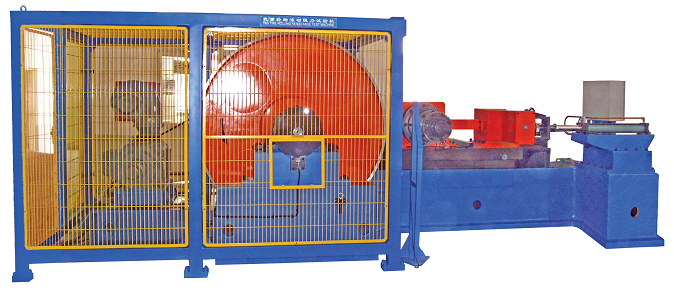
\includegraphics[width=\textwidth]{fig/2_rr_machine}
	\end{center}
	\caption{Máquina utilizada en los ensayos \textit{Rolling Resistance}. Fabricante:RPM. Modelo: TJRRRTBY. Especificaciones Técnicas: Anexo~\ref{apnd5}.}
	\label{fig:2_rr_machine}
\end{figure}

\subsubsection{Análisis dimensional}
El objetivo de este ensayo es verificar que
tanto las dimensiones generales de la cubierta,
como sus componentes internos
quedan dentro de la tolerancia de las especificaciones.

El ensayo se divide en 2 fases.
En la primera fase, El desarrollo de la cubierta es medido a la presión de
inflado especificada en el costado de la cubierta, y a un bar.
Mientras la cubierta conserva su presión de inflado especificada,
se toman los estampados de la huella del neumático introduciendo un folio A3 entre la superficie tintada del neumático, y la prensa.
En la segunda fase, se cortan y se pulen 3 secciones de la cubierta,
para posteriormente ser digitalizadas en un escáner de alta resolución.
Las mediciones a las imágenes obtenidas se realizan mediante un programa.

\subsection{OBJETIVOS}\label{sec_obj}
El objetivo de este trabajo es optimizar los recursos del
típico laboratorio de evaluación de neumáticos,
en el caso de un hipotético crecimiento de la demanda de ensayos.
Esto se consigue mediante el desarrollo de un método basado en una DES.

Para lograr el objetivo final se deberán completar los siguientes subobjetivos:

\begin{itemize}
	\item Modelar los procesos del LCP
		de acuerdo a los fundamentos de una DES,
		obteniendo un modelo ajustado a la realidad.
	\item Definir las variables independientes del proceso,
		que posteriormente serán usadas en la simulación.
	\item Estimar el tiempo de ciclo de cada proceso,
		a través de la asignación de
		distribuciones ajustadas a cada subproceso.
	\item Definir las variables dependientes
		que otorgara el sistema a la salida.
	\item Desarrollar un programa de simulación en el entorno de Python
		mediante el uso de la librería Simpy.
		Dicha simulación, será capaz de emular
		los distintos escenarios propuestos durante el desarrollo.
	\item Proponer una alternativa de la distribución de
		los recursos descritos al comienzo del trabajo, 
		para asegurar la capacidad del LCP cuando en el caso de que aumente la
		demanda de ensayos.
\end{itemize}

% **************************************************************************** %
%                                                                              %
%                                                         :::      ::::::::    %
%    sec_mteorico.tex                                   :+:      :+:    :+:    %
%                                                     +:+ +:+         +:+      %
%    By: acampo-p <acampo-p@student.42urduliz.com>  +#+  +:+       +#+         %
%                                                 +#+#+#+#+#+   +#+            %
%    Created: 2022/12/07 17:42:28 by acampo-p          #+#    #+#              %
%    Updated: 2023/02/16 03:09:08 by acampo-p         ###   ########.fr        %
%                                                                              %
% **************************************************************************** %

\section{MARCO TEÓRICO}

\subsection{SIMULACIÓN DE EVENTOS DISCRETOS}

Con el avance tecnológico experimentado desde los inicios de la computación,
nuevas maneras para afrontar la resolución de problemas han surgido,
que un siglo antes, habrían sido descartadas por su falta de viabilidad.
La capacidad de cálculo y el diseño de inteligencias artificiales,
ha proporcionado las herramientas necesarias
para solucionar aquellos problemas, que con métodos clásicos,
definitivamente demasiado complejos para modelar.
La simulación, hoy en día, es una de las tres metodologías consolidadas,
en el ámbito científico e ingenieril,
para la resolución de problemas \citep{banks1998handbook}.
Siendo esta metodología descrita como ``la técnica del último recurso'',
por \citet{garzia1986discrete},
debido a la intensa demanda computacional
que requería en el momento de su publicación,
el transcurso de los años ha mermado esta desventaja.

Diversos autores describen la simulación de la siguiente manera

\begin{itemize}
	\item ``Una simulación es
	el establecimiento de un modelo lógico-matemático de un sistema
	y la manipulación experimental de este en una computadora digital
	\citep{pritsker1974gasp}''.   
	\item ``La simulación es el proceso de diseñar
		el modelo de un sistema real y realizar experimentos
		con este modelo con el propósito de,
		entender el comportamiento del sistema,
		o evaluar distintas estrategias
		(dentro de los limites impuestos por un criterio
		o conjunto de criterios)
		para la operación del sistema'' \citep{shannon1976systems}.
	\item ``Una simulación es la imitación del modo de operación
		de un proceso real o sistema durante el transcurso del tiempo''
		\citep{banks1999introduction}.
\end{itemize}

Como se puede observar, el modelo,
es un término recurrente en el ámbito de la simulación.
\citet{banks1998handbook} sostiene que el modelo es la representación
del sistema simulado.
El autor matiza que la virtud de un modelo radica en su complejidad,
siendo necesario el balance entre una representación ajustada,
sin complicar en exceso el modelo.
Por tanto, aquellos factores que no influyan lo suficiente
en los resultados de la simulación, deberían ser eliminados,
ya que únicamente extienden el proceso de desarrollo.

El modelo, en consecuencia, constituye la base de la simulación,
define las variables, y criterios para las decisiones tomadas en la simulación.
\citet{banks1998handbook} señala,
la distinción entre un modelo matemático convencional
y el modelo de una simulación.
Los modelos matemáticos y estadísticos
suelen representar las variables de manera explícita,
relacionando variables independientes y variables dependientes
para obtener un resultado.
En el caso de una DES, el modelo utilizado se enfoca en
la representación de sus componentes internos y sus interacciones.

El funcionamiento de la DES, se basa en registrar los cambios
que van ocurriendo en el estado del sistema durante el transcurso del tiempo.
En el intervalo entre alternaciones de estado,
ocurren los eventos, propios de esta rama de simulación.
\citet{varga2001discrete} describe estos eventos como instantáneos,
siendo la duración de los mismos nula.
Durante el evento no ocurre nada especial,
salvo la alteración del estado del sistema.
Una sencilla representación de este concepto
puede ser observada en la Figura~\ref{fig:2_fc_simple_ex},
donde el sistema representado es un coche.
El coche posee 3 estados, los cuales se van sucediendo,
durante el transcurso del tiempo.

\begin{figure}[h]
	\begin{center}
		\includestandalone{fig/2_fc_simple_ex}
	\end{center}
	\caption{Representación del cambio de estado en una DES,
	los rectángulos representan el estado del sistema,
	mientras que las flechas indican el suceso de un evento instantáneo.}
	\label{fig:2_fc_simple_ex}
\end{figure}

\subsubsection{Terminología y funcionamiento de una DES}\label{TF_DES}

Para describir detalladamente este tipo de simulaciones,
es necesario definir previamente algunos conceptos.
Los siguientes conceptos
son la síntesis de la información redactada por \citet{banks1998handbook}
aplicados en el entorno de Python y su librería Simpy.

\paragraph{Las variables del estado}
del sistema proporcionan información
acerca de el comportamiento de los procesos
que se llevan a cabo durante la simulación.
Las variables de estado que el programa debe retornar
depende del objetivo del proyecto.
El programa deberá ser diseñado en torno a ellas,
puesto que, serán usadas
para el posterior cálculo de indicadores del rendimiento.
Un ejemplo es el momento de inicio y fin de un subproceso.

\paragraph{Las entidades}
son los objetos representados por el modelo.
Se distinguen dos tipos de entidades,
las dinámicas y las estáticas.
Las primeras avanzan en el sistema
a través de los procesos simulados, 
mientras que las segundas, dan servicio a las primeras
permaneciendo ocupadas en el proceso.
Considerando una gasolinera como sistema,
la entidad dinámica sería un coche repostando combustible,
mientras que la estática, sería la estación de repostaje.
Estos objetos pueden poseer atributos,
como el consumo de combustible o el tamaño de su depósito.
Dependiendo del objetivo de la simulación,
algunos atributos serán relevantes en diseño del modelo.

\paragraph{Un recurso}
es una entidad
que provee de servicio a una entidad dinámica.
Los recursos pueden servir a múltiples entidades simultáneamente.
De manera similar, una entidad puede
solicitar varios tipos de recursos en distintas cantidades.
Si la demanda de una entidad no se satisface,
esta entrará en una cola,
a la espera de la liberación del recurso.
Cuando la entidad tome el recurso,
lo mantendrá ocupado durante la duración del proceso.
Los recursos pueden tener varios estados,
como disponible, ocupado, averiado, en mantenimiento\ldots
Un ejemplo de recurso, puede ser el número de
estaciones de autoservicio que posee una gasolinera.

\paragraph{Una actividad}
es un periodo de tiempo,
el cual es conocido previo a su inicio.
Su duración puede ser determinada de varias maneras;
mediante una constante, una distribución estadística,
el resultado de una ecuación, un archivo o una decisión lógica.
El conocimiento de su duración,
supone saber cuando un recurso sera liberado,
lo que facilita el trabajo de computación.
Por ejemplo, un coche rellenando el depósito de combustible,
se puede modelar mediante una ecuación que relacione
el caudal de la estación de servicio con el tamaño del depósito del coche.
Este modelo devuelve la duración de la actividad, es decir,
el tiempo que tarda el coche en repostar.

\paragraph{Una demora}
es un periodo de espera indefinido
antes del comienzo de una actividad.
Este depende de la ejecución
del resto de actividades prioritarias,
por lo que el final de la espera no se puede determinar
mientras el recurso siga ocupado.
Relacionado con el ejemplo anterior, una demora,
puede representarse como la duración de la espera
del coche que esta a la cola de repostaje.

\paragraph{Un evento}
ocurre al principio y al final de una actividad o demora.
Marcan la transición del sistema de un estado a otro.
Véase un ejemplo en la Figura~\ref{fig:2_fc_simple_ex}.

Considerando todos estos conceptos,
las entidades del sistema compiten entre ellas por el uso de los recursos,
si estos no se encuentran disponibles, quedan a la espera de poder solicitarlos.
Tanto las actividades como las demoras reclaman estas entidades
durante los intervalos entre eventos,
siendo liberadas para el siguiente proceso una vez finalizado el periodo.
Una DES, puede describirse como el avance de una entidad o conjunto de entidades
a través  de las actividades que modelan el proceso real.
Este avance es accionado
mediante el transcurso de tiempo virtual dentro de la simulación.
Véase un ejemplo en la Figura~\ref{fig:2_fc_simple_ex}.

\subsubsection{Exposición de un caso ficticio usando una DES}\label{example_descrp}

Con el objetivo de ilustrar los conceptos descritos en la sección~\ref{TF_DES}
y demostrar la capacidad de resolución de problemas de la DES,
se ha procedido a emular un caso práctico.

Supóngase que un ayuntamiento ficticio desea disminuir
los problemas causados por el congestionamiento del tráfico en la ciudad.
El ayuntamiento solicita a una consultoría ingenieril
desarrollar un proyecto para observar el
desempeño de las distintas soluciones planteadas.
La consultoría ve apropiado usar una DES para valorar
el impacto de las distintas propuestas
y proponer un plan de acción óptimo a la entidad contratante.

El objetivo principal del ayuntamiento es
minimizar la cantidad de vehículos que circulan por la ciudad.
Una de las causas de congestión apunta a una estación de repostaje
con unos precios particularmente competitivos
que causa complicaciones a la entrada de la ciudad.
Se cree que su capacidad de abastecimiento
no es suficiente durante los picos de alta actividad.
Por otra parte, la ciudad es un potente centro de actividad comercial.
Muchos empleados se desplazan a diario en coche,
lo que sumado a los espacios limitados de estacionamiento,
y la alta densidad poblacional,
hace sospechar que los conductores se demoran en exceso
a la hora de buscar aparcamiento.
Se teme que este tiempo adicional,
sea un factor considerable en las emisiones totales de los vehículos.

Con las siguientes dos medidas se espera obtener
una reducción del congestionamiento del tráfico en la ciudad.

\begin{itemize}
	\item Primeramente, negociar un ampliamiento
		del servicio de distribución de combustibles
		con la empresa propietaria de la estación de repostaje.
	\item Paralelamente, ampliar la capacidad de un \textit{parking}
		público gratuito ubicado cerca del núcleo de actividad laboral.
\end{itemize}

La simulación planteada, tratará de emular el comportamiento de los vehículos
que circulan por la ciudad durante el transcurso de una jornada laboral normal.
Es por ello que el comienzo de la simulación se estima en torno a las 7:00 a.m.
y se prologa hasta 9:00 p.m.
El modelo producirá 2 tipos de entidades,
el vehículo de tipo `A',
que será el medio de transporte para los trabajadores de la zona,
y el de tipo `B' que englobará todo tipo de usuarios ajenos al ámbito laboral.
Esta distinción se ha considerado necesaria,
debido a la uniformidad que representa el primer grupo, respecto al segundo, algo más caótico.
Los vehículos generados seguirán la rutina descrita en la Figura~\ref{fig:2_fc_complex_ex}.

\begin{figure}
	\begin{center}
		\includestandalone{fig/2_fc_complex_ex}
	\end{center}
	\caption{Modelo del caso práctico descrito en el apartado~\ref{example_descrp}}
		\label{fig:2_fc_complex_ex}
\end{figure}

La consultoría, por una parte, establece
las propiedades generales de su modelo en la Tabla~\ref{tab:2_tbl_spec01_ex}.
Mientras que, por otra parte, decide recopilar información clave
para el desarrollo del modelo de simulación.
A raíz de un análisis obtiene los datos mostrados en la Tabla~\ref{tab:2_tbl_spec02_ex}.

\begin{table}
	\centering
	\caption{Especificaciones generales.}
	\documentclass[varwidth=\maxdimen]{standalone}
\usepackage[utf8]{inputenc}
\usepackage[spanish]{babel}
\usepackage{booktabs}

\begin{document}

\begin{tabular}{ l c }
	\toprule
	Nombre	& Valor	\\
	\midrule
	Duración				& 960	min \\
	Ejecuciones				& 20	uds. \\
	Capacidad del parking	& 100	uds. \\
	Estaciones de repostaje	& 4		uds. \\
	Probabilidad de repostaje		& 50\% \\
	\bottomrule
\end{tabular}

\end{document}

	\label{tab:2_tbl_spec01_ex}
\end{table}
	
\begin{table}
	\centering
	\caption{Propiedades de las distribuciones observadas en los procesos reales.}
	\documentclass[varwidth=\maxdimen]{standalone}
\usepackage[utf8]{inputenc}
\usepackage[spanish]{babel}
\usepackage{booktabs}

\begin{document}

\begin{tabular}{ l c c c }
	\toprule
	Variable	& Tipo de vehículo	& Distribución	& Constantes (min) \\
	\midrule
	Conducir largo	& A y B	& Gamma			& $k = 8$, $\theta = 3$ \\
	Conducir corto	& A y B	& Triangular	& $min = 2$, $moda = 3$, $max = 4$ \\
	Buscar \textit{parking}	& A y B	& Gamma			& $k = 10$, $\theta = 1$ \\
	Repostar		& A y B	& Triangular	& $min = 4$, $moda = 5$, $max = 8$ \\
	Entre llegadas	& A*	& Exponencial	& $\lambda = 1$ \\
					& B		& Exponencial	& $\lambda = 15$ \\
	Estacionamiento	& A		& Normal		& $\mu = 560$, $\sigma = 60$ \\
					& B		& Lognormal		& $\mu = 5$, $\sigma = 0.7$ \\
	\bottomrule
\end{tabular}

\end{document}

	\footnotesize{*La generación de entidades tipo `A' únicamente
		se prolonga desde el comienzo de la simulación hasta el minuto 150.
	Así, se obtiene una aproximación, al horario típico de un día laboral.}
	\label{tab:2_tbl_spec02_ex}
\end{table}

Como puede observarse en la Figura~\ref{fig:2_fig_example_01},
la adición de 2 estaciones de autoservicio en la gasolinera
evita su colapso en intervalos críticos.
En el gráfico situado a la izquierda,
el pico de actividad azul
en torno al minuto 150 de la ejecución de la simulación,
se ve drásticamente reducido,
mientras que el repunte secundario es completamente eliminado.
A su vez, en el gráfico adyacente,
La desviación estándar de tiempos de espera queda reducida
y su media queda desplazada hacia el eje.

\begin{figure}
	\begin{center}
		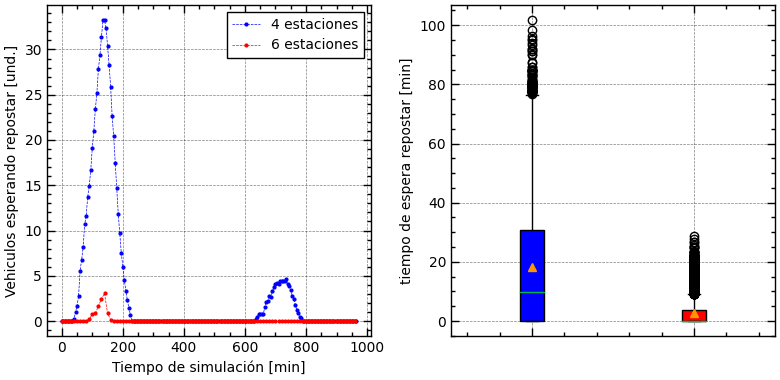
\includegraphics[width=\textwidth]{fig/2_fig_example_01}
	\end{center}
	\caption{Izquierda: Evolución de los vehículos a la espera de repostar para distintos escenarios. Derecha: Distribución de los tiempos de espera de repostaje para los distintos escenarios}
	\label{fig:2_fig_example_01}
\end{figure}

Continuando con el análisis, en la Figura~\ref{fig:2_fig_example_02},
El efecto de incrementar en un 50\% las plazas de parking disponible,
no es apreciable en el gráfico expuesto arriba.
La cantidad de vehículos en carretera permanece similar,
mientras que en el gráfico inferior los vehículos saturan el \textit{parking}
hasta su nuevo límite.
Al no haber una clara correlación entre ambos indicadores,
se ilustra la representación de la distribución de tiempos de conducción
en la Figura~\ref{fig:2_fig_example_03}.
En esta exposición, puede llegar a apreciarse una ligera diferencia en los tiempos de conducción,
aunque un test de hipótesis sería necesario
para determinar si estas diferencias son estadísticamente significativas.

En conclusión, los resultados muestran una clara ruta de inversión
a la hora de ampliar la estación de combustibles,
mientras que la expansión del \textit{parking} parece irrelevante.
Esto demuestra la capacidad de recopilación de datos que ofrece una DES.
Simultáneamente subraya la importancia del tratamiento de los datos obtenidos,
y el uso de pruebas estadísticas, para la obtención de conclusiones certeras.

\begin{figure}[H]
	\begin{center}
		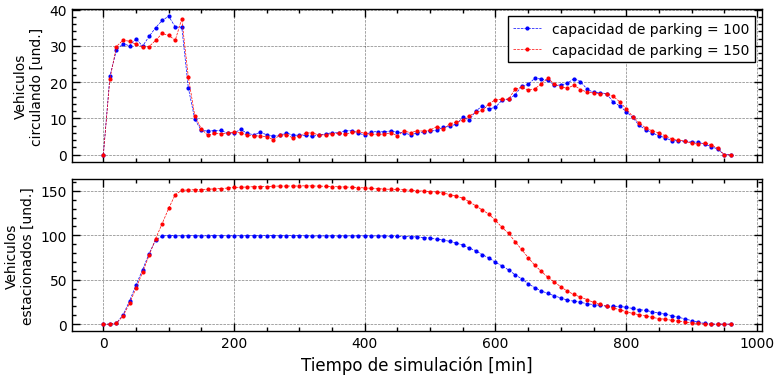
\includegraphics[width=\textwidth]{fig/2_fig_example_02}
	\end{center}
	\caption{Evolución de la cantidad de vehículos a lo largo de la simulación, en distintos escenarios. Arriba: Vehículos en circulación. Abajo: Vehículos estacionados.}
	\label{fig:2_fig_example_02}
\end{figure}

\begin{figure}[H]
	\begin{center}
		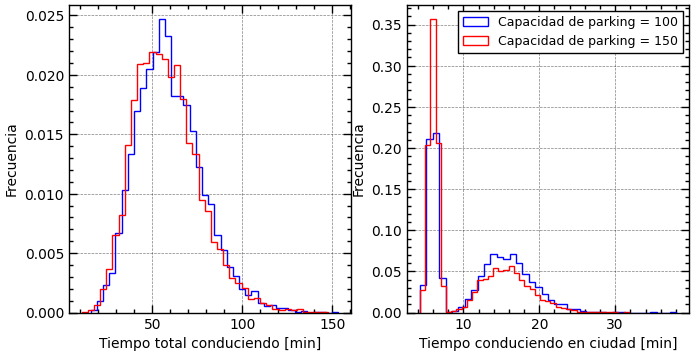
\includegraphics[width=\textwidth]{fig/2_fig_example_03}
	\end{center}
	\caption{Distribución del tiempo de conducción para distintos escenarios. Izquierda: Tiempo total en circulación. Derecha: Tiempo circulando dentro de la ciudad.}
	\label{fig:2_fig_example_03}
\end{figure}

\subsubsection{Etapas de desarrollo de una DES}

Para que un proyecto tan complejo como una DES prospere, es fundamental estructurarlo.
El diagrama expuesto en la Figura~\ref{fig:2_fc_sim_cookbook}
publicado por \citet{banks1998handbook}
define las etapas que deberían seguir este tipo de proyectos.
Al ser este proyecto un simple Trabajo de Fin de Grado,
este esquema servirá como orientación, más que como plano para la construcción de la simulación.
Por ejemplo, la recopilación de datos ha resultado imposible en el momento de redacción del trabajo,
pero se espera desarrollar el proyecto
a partir de las más ajustadas distribuciones de probabilidad supuestas
para el desarrollo del modelo.
Se espera que este trabajo asiente una base,
y que las imperfecciones actuales puedan ser corregidas en el futuro.

\begin{figure}
	\begin{center}
		\includestandalone{fig/2_fc_sim_cookbook}
	\end{center}
	\caption{Esquema del proceso de desarrollo de una DES.}
	\label{fig:2_fc_sim_cookbook}
\end{figure}

\paragraph{Formulación del problema, establecimiento de objetivos, y plan general.}

Cada DES comienza con la declaración del problema que se tratará de solucionar.
Esta etapa es crucial debido a que el resto del
trabajo se asentara sobre esta base.
Se debe asegurar que el problema que se está formulando sea el correcto,
la comunicación entre el cliente y el equipo desarrollador debe ser óptima.
Una descripción precisa y un conocimiento extenso del sistema son necesarios para evitar
trabajar en solucionar el problema equivocado.
Es por ello que debe haber comunicación y \textit{feedback}
constante entre cliente y equipo.

En el caso de este trabajo, algo similar sucede.
Al ser un único autor, la comunicación no será un factor importante,
pero esto conllevara otras complicaciones.
El autor debe, comprender profundamente el sistema a modelar, y a su vez,
dominar el uso de las herramientas de simulación.
Manejar ambas, requerirá recordar la formulación del problema inicial
más frecuentemente para no desviarse de la dirección.

Respecto a los objetivos, estos deben ayudar a
asentar la dirección de trabajo actuando como plan general.
El establecimiento de varios objetivos alcanzables,
cohesivos y correctamente secuenciados,
guiará el proceso de desarrollo.
Estos objetivos quedan listados en la sección~\ref{sec_obj}.

\paragraph{Conceptualización del modelo.}\label{sec:modelconcept}

El sistema propuesto sugiere conceptualizar el modelo en orden inverso,
es decir, comenzar identificando los objetivos del proyecto,
tal y como se ve en la Figura~\ref{fig:2_fc_model_concept}.

\begin{figure}[h]
	\begin{center}
		\includestandalone{fig/2_fc_model_concept}
	\end{center}
	\caption{Diagrama de pasos a seguir en la conceptualización de un modelo.}
	\label{fig:2_fc_model_concept}
\end{figure}

El siguiente paso es hallar las preguntas clave a las que
se les quiere dar respuesta.
Generar una lista, y ordenar las preguntas respecto a su relevancia es lo ideal.
Además, cuantificar los beneficios asociados a estas, aclara su jerarquía.

Después, se debe determinar que outputs son necesarios
para contestar a las preguntas previamente formuladas.
Introduciendo en la simulación únicamente la complejidad necesaria,
agilizará el proceso de desarrollo y mantendrá el enfoque original.

Continuando con el alcance de la simulación,
se deben detallar los procesos críticos en el cálculo del \textit{output},
descartando o simplificando aquellos que no tengan gran impacto en la salida.
Por ejemplo, modelar recursos abundantes en la simulación,
no tendrá impacto en el retorno,
mientras que conocer los tiempos de espera de un proceso si lo hará.

Se Finaliza, especificando las variables independientes
que se introducirán al sistema.
Estas variables tienen que ser de alta calidad, ya que,
de lo contrario su introducción puede perjudicar al sistema al completo.
Un ejemplo seria el de distinguir entre distintas distribuciones
para entidades con atributos pobremente caracterizados.

\paragraph{Recopilación de datos.}

Cualquier DES requiere datos. La recopilación de la información del sistema,
o la estimación en caso de ser un sistema ficticio, es una necesidad.

El primer paso es recopilar la información de la que se dispone actualmente.
En el caso de no poseer información, o de que los datos presenten sesgos,
se deben medir las características necesarias.
Finalmente, en caso de resultar imposible la medición,
se deben tomar como referencia las opiniones de un experto,
que normalmente suele ser el operario que maneja la máquina.

\paragraph{Traducción del modelo.}

El modelo de simulación se construye a partir de la información desarrollada en el anterior punto.
Este proceso consiste en traducir de manera eficaz el esqueleto previamente desarrollado,
a un lenguaje que el ordenador pueda procesar.
Para ello, \citet{banks1998handbook} sugiere lo siguiente:

\begin{itemize}
	\item Enfoque en el problema. El proyecto no debería limitarse a desarrollar el modelo,
		sino que debería tratar de invertir aproximadamente el mismo tiempo
		en la exploración del sistema y la solución de problemas.
	\item Comienzo simple. El comienzo del proyecto debe ser simple,
		adquiriendo complejidad hasta alcanzar el detalle necesario.
	\item Manejo de la inteligencia del modelo.
		El modelo no debe superar el rendimiento de los procesos reales.
		El modelo desarrollado puede desarrollar ventajas respecto a su contrapartida real,
		como conocer la ubicación exacta de una pieza instantáneamente.
		Los humanos que gestionan el proceso difícilmente van a poder lograr este control,
		y supondrá una característica inalcanzable en el sistema real.
	\item Revisión. Revisar el funcionamiento del proyecto frecuentemente.
		Esto evitará desvíos respecto al objetivo principal
		y facilitara el proceso de verificación y validación.
\end{itemize}
\paragraph{Verificación y validación.}

Comprobar el correcto funcionamiento de la DES es fundamental.
Esta es la labor de la verificación y validación (VV).
\citet{banks1998handbook} sugiere que este paso se realice
frecuentemente a lo largo del proceso de desarrollo.
Esto evita complicaciones una vez el proyecto se vuelve demasiado extenso y demasiado complejo.
Realizar la VV en cada pieza funcional del modelo
cada vez que suceda algún cambio es lo recomendable.

Por una parte, la verificación es el proceso encargado de
comprobar que la simulación se ejecute de la manera esperada.
En este proceso se intentará hallar errores en el programa.
Esto se logra comprobando que la ejecución de cada paso
en la simulación sea la correcta y retorne los resultados esperados.

Por otra parte, la validación consiste en comparar,
el comportamiento del modelo respecto al comportamiento real del sistema.
En el caso de poseer datos sobre el sistema simulado,
el libro sugiere utilizar herramientas estadísticas como,
el test \textit{t} de Student o
análisis de regresión donde el ajuste a la realidad será comprobado.
En el caso de no poseer los datos del sistema,
se optara por un enfoque cualitativo.
Aunque no haya datos, el comportamiento de un sistema
puede predecirse cualitativamente, al cambiar ciertas variables.
Por ejemplo en un tanque de agua cilíndrico,
aunque el volumen del tanque y el caudal de entrada del agua sea desconocido,
el nivel del agua disminuirá si el flujo neto es negativo.
Si el programa ejecutado obtiene el resultado contrario,
este sera invalidado comenzando la revisión del mismo.

\paragraph{Análisis.}

Mediante el análisis del el retorno de la simulación,
se obtienen las conclusiones a las preguntas plateadas al inicio del proyecto.
Primeramente, se deberán plantear los distintos escenarios que serán simulados.
Estos escenarios serán ejecutados en la simulación
obteniendo sus variables de salida.
El correcto tratamiento de los datos,
junto con una exposición significativa de ellos dará claridad a los resultados.
No obstante, para obtener las conclusiones deseadas,
deberán realizarse test estadísticos a los resultados para certificarlos.

\paragraph{Documentación y comunicación.}

Con la intención de que este proyecto
pueda ser continuado en el futuro por otra persona,
la documentación se vuelve necesaria.
El proyecto se considera documentado,
por una parte, mediante este trabajo,
y por la otra mediante un código fuente autoexplicativo,
con abundantes comentarios.

\subsection{TEORÍA DE LA PROBABILIDAD Y DES}

La probabilidad está estrechamente relacionada con la DES.
Previamente a comenzar el proceso de formulación del modelo de una DES,
los datos empíricos medidos en los procesos reales
se traducen a un modelo reproducible computacionalmente.
A este ejercicio se le denomina comúnmente como
ajuste de distribución de probabilidades.
Estas distribuciones de probabilidades son
continuamente usadas durante la simulación,
con el fin de representar la aleatoriedad de
las actividades que se llevan a cabo.
Cada vez que un sucede un evento en la simulación,
se toma una muestra de su distribución de probabilidad asociada.
Esta muestra o variable aleatoria corresponde a la duración de dicha actividad.
Concatenando la sucesión de eventos,
se consigue replicar la aleatoriedad del sistema.

El uso de la teoría de la probabilidad no acaba aquí.
Una vez finalizada la etapa de simulación,
los datos obtenidos de la simulación son puestos a prueba.
Para evitar obtener conclusiones erróneas,
debido a un resultado excepcional al azar,
se realizan múltiples ejecuciones de la simulación.
Los resultados obtenidos son una población de
las variables dependientes calculadas por la simulación.
El método más común para determinar la diferencia
entre los distintos escenarios simulados es el test de hipótesis.

\subsubsection{Variables aleatorias o random}

Según \citet{meester2008natural},
una variable aleatoria ($X$) puede explicarse
como un número cuyo valor no es conocido en el momento de su planificación.
Aunque el valor último de esta variable sea desconocido,
el rango de valores que pueden tomar estas variables
viene determinado por una función.
A esta función se le denomina Función de Distribución de Probabilidad (FDP).

\subsubsection{Distribuciones de probabilidad}\label{sec_prob_dist}

Una distribución de probabilidad es una función estadística
que determina la probabilidad de que una variable aleatoria 
\citep{simon2002probability},
obtenga los valores posibles que contiene la propia distribución.
Las FDP comúnmente usadas
en los modelos de una DES son las siguientes:

\paragraph{Distribución uniforme.} Esta distribución
destaca debido a que los valores, dentro de un rango definido,
tienen la misma probabilidad de ser escogidos.
Suele ser usada para proporcionar peso
a los distintos sucesos que forman una lista.
Por ejemplo, para representar la probabilidad de
que un coche tenga matrícula palíndroma,
se puede emplear una distribución uniforme de $a=0$ y $b=9999$.
Para cualquier número obtenido inferior a 904,
la matrícula del coche se determina palíndroma.

\begin{equation}
	P(x) = \frac{1}{b-a}
\end{equation}

\paragraph{Distribución normal.} Aparece continuamente
en fenómenos naturales, sociales y psicológicos.
Es la más común de las distribuciones
y sus parámetros son sencillos e intuitivos.
La condición que se debe cumplir para poder usar esta FDP,
es que los datos que forman un conjunto
deben ser independientes entre sí.
Por ejemplo, la vida útil de un modelo de coche
puede representarse mediante esta distribución.

\begin{equation}
	P(x) = \frac{1}{\sqrt{2 \pi \sigma ^{2}}} e^{-\frac{(x-\mu)^{2}}{2\sigma ^{2}}}
\end{equation}

\paragraph{Distribución lognormal.} Sucede cuando al aplicarle
un logaritmo a una variable aleatoria,
esta acaba normalmente distribuida.
Si la variable aleatoria es $e^X$, $X$
sigue una distribución normal.
Esta FDP presenta una asimetría positiva,
lo que la hace idónea para representar procesos
en los que normalmente su duración se encuentra
dentro de un intervalo previsto,
pero que puede llegar a extenderse más de lo normal en el tiempo.
Por ejemplo, la duración de la reparación de un coche
pude ser modelada por esta FDP.
Una reparación puede llegar a extenderse debido a
imprevistos como la falta de piezas de recambio,
o problemas inicialmente no detectados.

\begin{equation}
	P(x) = \frac{1}{\sigma x \sqrt{2 \pi}} e^{-\frac{(ln(x)-\mu)^{2}}{2\sigma ^{2}}}
\end{equation}

\paragraph{Distribución triangular.} Se caracteriza por estar limitada,
entre un límite inferior $a$, y otro superior $b$,
siendo su valor más probable la moda $m$.
A menudo es usada cuando no se dispone de
suficientes datos de un proceso.
Por ejemplo, en un taller no se dispone de datos sobre
lo que un mecánico se demora en cambiar una rueda a un coche,
pero el propio mecánico, por experiencia,
sabe aproximadamente el mínimo, el máximo, y la duración típica. 

\begin{equation}
	P(x;a,m,b) =
	\begin{cases}
		\frac{2(x-a)}{(b-a)(m-a)}	&\text{para $a\leq x\leq m$,} \\
		\frac{2(b-x)}{(b-a)(b-m)}	&\text{para $m\leq x\leq b$,} \\
		0							&\text{para el resto}
	\end{cases}
\end{equation}

\paragraph{Distribución exponencial.} Es la distribución
de la probabilidad del tiempo entre eventos de un proceso de Poisson.
Un proceso de Poisson se caracteriza por que los eventos
ocurren continuamente y de manera independiente.
En las DES, se usa para determinar el tiempo entre llegadas
de las entidades generadas.
$\lambda$ es el parámetro que marca la frecuencia de las llegadas.
Por ejemplo, en un taller los clientes llegan uno detrás de otro,
el periodo entre estas llegadas puede ser modelado mediante esta FDP.

\begin{equation}
	P(x; \lambda) =
	\begin{cases}
		\lambda e^{-\lambda x}	& x \geq 0, \\
		0										& x < 0
	\end{cases}
\end{equation}

\paragraph{Distribución gamma.} Es una distribución de probabilidad de
2 parámetros, constituyéndose por el parámetro de forma $k$,
y la escala $\theta$. Debido a sus parámetros,
es adecuada para el ajuste de distribuciones cuando las variantes
de distribuciones normales no se ajustan a el conjunto de datos.
Permite representar una asimetría en la distribución.

\begin{equation}
	P(x) = x^{k-1} \frac{e^{-x/\theta}}{\theta ^{k}\Gamma (k)}
	\text{, siendo:}
	\Gamma (k) = (k-1)!
\end{equation}

\subsubsection{Test de hipótesis}\label{sec_test_est}

La comprobación de los resultados obtenidos en las DES,
es una parte fundamental de la simulación.
Para ello se suelen emplear los test de hipótesis como muestra de la validez
de las conclusiones obtenidas.

El test de hipótesis involucra formular,
2 o más hipótesis, que serán puestas a prueba
mediante el empleo de test estadísticos \citep{martin2022introduction}.
Aplicado a el caso desarrollado en este trabajo,
se trata de comprobar las hipótesis formuladas
mediante la comparación de las poblaciones obtenidas en distintos escenarios.

Un formato común en el ámbito de test de hipótesis es el siguiente:

\begin{itemize}
	\item Hipótesis nula, $H_0$, trata de demostrar que el fenómeno observado es únicamente resultado del azar.
	\item Hipótesis alternativa, $H_1$, trata de demostrar la hipótesis que se desea probar. Existen 3 tipos:
		\begin{itemize}
			\item parámetro de población $>$ valor hipotetizado.
			\item parámetro de población $<$ valor hipotetizado.
			\item parámetro de población $\neq$ valor hipotetizado.
		\end{itemize}
\end{itemize}

Para realizar un test de hipótesis,
primero debe escogerse un test,
y aplicarlo a las muestras de la población a analizar.
Después, la hipótesis nula es rechazada o no dependiendo
del valor \textit{p} obtenido.

Un test de hipótesis muy usado es el test \textit{t}
de Student~\eqref{eq:tstudent}.

\begin{equation}
	t = \frac{\tilde{x} - \mu_0}{s / \sqrt{n}}
	\label{eq:tstudent}
\end{equation}

El valor \textit{p}, es la probabilidad condicional de
los valores a los extremos de un test estadístico,
asumiendo que la hipótesis nula es cierta.
Por convención, si la probabilidad de la hipótesis nula es $<5\%$, o $<0.05$,
la hipótesis nula es rechazada.
De lo contrario, no es posible rechazar la hipótesis nula,
lo que no supone que esta sea cierta.

% **************************************************************************** %
%                                                                              %
%                                                         :::      ::::::::    %
%    sec_resultados.tex                                 :+:      :+:    :+:    %
%                                                     +:+ +:+         +:+      %
%    By: acampo-p <acampo-p@student.42urduliz.com>  +#+  +:+       +#+         %
%                                                 +#+#+#+#+#+   +#+            %
%    Created: 2022/12/07 17:42:28 by acampo-p          #+#    #+#              %
%    Updated: 2023/02/10 03:54:54 by acampo-p         ###   ########.fr        %
%                                                                              %
% **************************************************************************** %

\section{RESULTADOS}

Una vez simulados los distintos escenarios,
se ha procedido a analizar las tablas de datos obtenidos por la simulación.

\begin{table}
	\centering
	\caption{Capacidad máxima de ensayos por maquina.}
	\documentclass[varwidth=\maxdimen]{standalone}
\usepackage[utf8]{inputenc}
\usepackage[spanish]{babel}
\usepackage{booktabs}

\begin{document}

\begin{tabular}{ l c }
	\toprule
	Ensayo & Capacidad máxima (unds.) \\
	\midrule
	\textit{Endurance}	& 934 \\
	\textit{Rolling Resistance}		& 2502 \\
	\bottomrule
\end{tabular}

\end{document}

	\label{tab:4_tbl_max_cap}
\end{table}

En la Figura~\ref{fig:4_hist_tests_done} se han graficado
las distribuciones de el numero de ensayos realizados, en un año simulado,
para cada escenario.
Cada escenario ha sido ejecutado 100 veces, y se ha trazado la frecuencia
con la que ocurría un determinado numero de ensayos en el histograma.
La figura consta de 2 gráficas,
correspondiendo el histograma (A) a los ensayos Endurance
y el histograma (B) a los ensayos Rolling.
De izquierda a derecha se pueden observar 4 distribuciones de distintos colores.
Cada uno de ellos corresponde a una configuración de turnos
del técnico encargado de estas maquinas.
Los turnos en los cuales el operario esta disponible como recurso
van desde 1 a tiempo completo, incluidos los fines de semana.

En el histograma superior puede observarse la distinción
que ocurre entre las distintas configuraciones.
Cada configuración tiene un amplio rango de ensayos,
mostrando el comportamiento estocástico de este tipo de ensayos.
Exceptuando la configuración a tiempo completo,
la cantidad de ensayos, parece variar dentro de un rango común de 100 ensayos.
Esta tendencia cambia al disponer a tiempo completo
de un operario que monte la maquina.
Al eliminarse la posibilidad
de que el ensayo finalice fuera del horario laboral,
la desviación estándar de ensayos realizados se reduce al mismo tiempo
que la media de ensayos se aproxima a la capacidad ideal.

En el histograma inferior,
las 3 primeras configuraciones expuestas,
muestran un comportamiento similar observado en
la configuración a tiempo completo, observada en el anterior gráfico.
Esto se debe, a que el técnico solamente puede llegar a lanzar
un determinado numero de ensayos por turno trabajado.
Esta cantidad se mantiene uniforme a lo largo de las ejecuciones
debido a que la duración de este ensayo es inferior
a la duración del turno del técnico.
Mientras el horario de trabajo sea limitado
la tendencia de ensayos corresponderá a la ecuación~\ref{eq:testdone}.
En el escenario en el que el técnico esta disponible durante 3 turnos al día,
la acumulación de eventos aleatorios se vuelve notable
en la desviación de ensayos observada respecto a los anteriores 2 escenarios.
Finalmente, a tiempo completo, la desviación estándar
aumenta considerablemente, ya que no hay un descanso
que regule la aleatoriedad de los ensayos.

\begin{equation}
	Test Realizados = 365 \cdot 8 \cdot 
	\underbrace{
		\left(\frac{N_{turnos}}{\mu_{test}} + 1\right)
	}_{\text{Entero truncado}}
	\label{eq:testdone}
\end{equation}

Una representación mas significativa ocurre
cuando se normaliza la cantidad de ensayos respecto
a la capacidad máxima de trabajo.
De esta marera, se obtiene la fracción de tiempo de utilización de maquina
representado en la Figura~\ref{fig:4_hist_time_sat}.
Esta conversión logra asentar la base necesaria para
comparar el grado de utilización de maquinas de manera directa.

\begin{figure}
	\begin{center}
		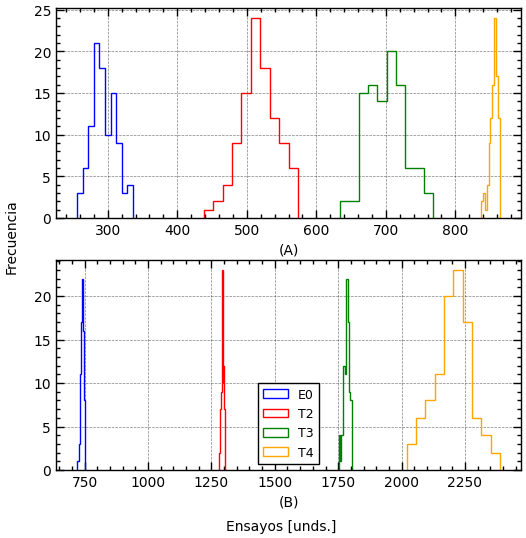
\includegraphics{fig/4_hist_tests_done}
	\end{center}
	\caption{Distribución de ensayos realizados para los escenarios descritos en la leyenda.
	(A) Ensayos endurance. (B) Ensayos rolling.}
	\label{fig:4_hist_tests_done}
\end{figure}

\begin{figure}
	\begin{center}
		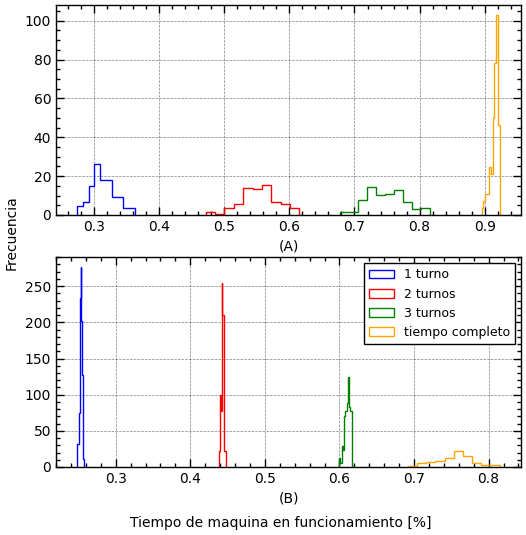
\includegraphics{fig/4_hist_time_sat}
	\end{center}
	\caption{Distribución de el nivel de saturación en tiempo de lo escenarios descritos en la leyenda.
	(A) Ensayos endurance. (B) Ensayos rolling.}
	\label{fig:4_hist_time_sat}
\end{figure}

\begin{table}
	\centering
	\caption{Media y desviación estándar de ensayos realizados por cada escenario y tipo de ensayo.}
	\documentclass[varwidth=\maxdimen]{standalone}
\usepackage[utf8]{inputenc}
\usepackage[spanish]{babel}
\usepackage{booktabs}
\usepackage{multirow}

\begin{document}

\begin{tabular}{ l c c c c }
	\toprule
	Escenario &
	\multicolumn{2}{c}{Ensayos \textit{Endurance} (unds.)} &
	\multicolumn{2}{c}{Ensayos \textit{Rolling Resistance} (unds.)} \\
		& $\mu$		& $\sigma$	& $\mu$		& $\sigma$ \\
	\midrule
	E0	& 293.35    & 17.27		& 739.35	& 5.51 \\
	T2	& 516.83	& 26.38		& 1293.40	& 5.00\\
	T3	& 701.07	& 27.25		& 1782.26	& 11.15 \\
	T4	& 855.06	& 5.70		& 2202.28	& 73.18 \\
	\bottomrule
\end{tabular}

\end{document}

	\label{tab:4_tbl_test_done}
\end{table}

Si se grafica la fracción de tiempo de utilización de maquina,
respecto a la fracción del tiempo trabajado,
con los escenarios expuestos hasta ahora,
se obtiene la Figura~\ref{fig:4_sctr_time_sat}.
La dispersión de los datos se ajusta perfectamente a una regresión lineal
a partir de la fracción de tiempo trabajado de 0.25 en adelante.
Para ambas maquinas, la relación entre ensayos realizados
y tiempo trabajado es directamente proporcional.
La obtención de esta relación,
junto con las capacidades máximas de las maquinas
expuestas en la tabla~\ref{tab:4_tbl_max_cap} permite 
anticipar si la capacidad del LCP será suficiente
para saciar la demanda de ensayos.

Teniendo en cuenta los datos obtenidos a través de la regresión lineal,
la ecuación~\ref{eq:qced} modela la cantidad de ensayos endurance
realizados en función a la fracción de horas trabajadas en un año.
Siendo la fracción de horas trabajadas descrita como la ecuación~\ref{eq:f_hours}.
A su vez, la ecuación~\ref{eq:rr} aplica la misma función
pero para los ensayos rolling.
Para un determinado objetivo de test realizados,
las ecuaciones mencionadas pueden resolverse
para obtener la cantidad de horas necesarias para llegar al objetivo.
En el caso de requerir más horas de las que una jornada laboral normal dispone,
se propone completar dichas horas sobrantes
reposicionando uno de los técnicos en un turno adicional durante un periodo.
Dicho periodo se puede calcular mediante la ecuación~\ref{eq:period},
de esta manera se aprovechan al máximo los recursos humanos disponibles.
Para ello primeramente se calcula
el máximo de turnos anuales mediante la ecuación~\ref{eq:gf}.

\begin{equation}
	Test Realizados = 934 \cdot 0.79 \cdot f_{t trabajo} + 0.15
	\label{eq:qced}
\end{equation}

\begin{equation}
	Test Realizados = 2502 \cdot 0.66 \cdot f_{t trabajo} + 0.12
	\label{eq:rr}
\end{equation}

\begin{equation}
	f_{t trabajo}= \frac{t_{trabajo}}{365~\frac{\text{días}}{\text{año}} \cdot
	24~\frac{\text{horas}}{\text{días}}}
	\label{eq:f_hours}
\end{equation}

\begin{equation}
	\begin{array}{c}
		G(f_{t trabajo}) = f_{t trabajo}
		\frac{365~\text{días}
		\cdot 24~\frac{\text{horas}}{\text{días}}}
		{8~\frac{\text{horas}}{\text{días}} \cdot
			5~\frac{\text{días}}{\text{semanas}} \cdot
		52~\frac{\text{semanas}}{\text{año}}} \\
		\\
		Turnos= 
		\begin{cases}
			1	& G(f_{t trabajo}) \leq 1 \\
			2	& 1 < G(f_{t trabajo}) \leq 2 \\
			3	& 2 < G(f_{t trabajo}) \leq 3 \\
			4	& G(f_{t trabajo}) > 3
		\end{cases}
	\end{array}
	\label{eq:gf}
\end{equation}

\begin{equation}
	Periodo = 12~\text{meses} \cdot (G(f_{t trabajo}) - Turnos -1)
	\label{eq:period}
\end{equation}

\begin{figure}
	\begin{center}
		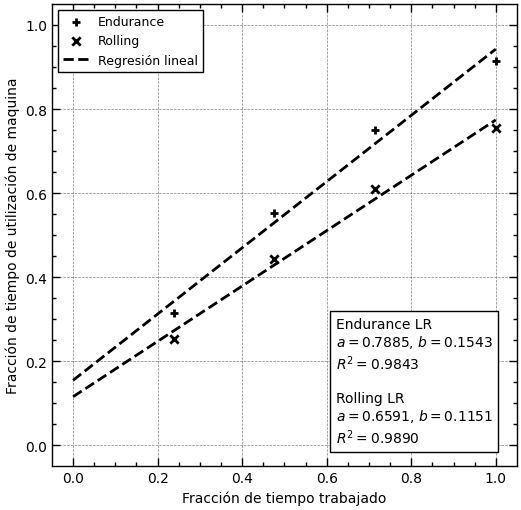
\includegraphics{fig/4_sctr_time_sat}
	\end{center}
	\caption{Tendencia proporcional del aumento del numero de ensayos al añadir turnos de trabajo.}
	\label{fig:4_sctr_time_sat}
\end{figure}

Con el fin de descartar otro tipo de configuraciones,
como múltiples técnicos trabajando simultáneamente,
se ha graficado la Figura~\ref{fig:4_box_techn1-2_comp}.
La diferencia en ambos ensayos parece mínima,
pero con la intención de descartar la idea de que
2 técnicos trabajando simultáneamente incrementa el numero de ensayos realizados,
se desarrolla el siguiente test de hipótesis.

\begin{itemize}
	\item $H_1$: $\mu_1 \neq \mu_2$
	\item $H_0$: $\mu_1 = \mu_2$
\end{itemize}

Se ha tratado de descartar la hipótesis nula mediante la prueba de valor-p,
y test t-student.
Los resultados de la prueba,
han sido recogidos en la tabla~\ref{tab:4_tbl_studet-t}.
El bajo valor-p obtenido en ambos tipos de ensayo
descarta la hipótesis nula formulada anteriormente.
Esto significa que las distribuciones
tienen una diferencia estadísticamente significativa.
A un siendo este el caso,
el escenario en el que se trabaja a 2 turnos,
es definitivamente superior,
como se puede observar en la Figura~\ref{fig:4_box_techn1-2_comp}.
Al consumir ambos la misma cantidad de recursos,
esto descarta la configuración en la que 2 técnicos trabajan simultáneamente.

\begin{table}
	\centering
	\caption{Resultados del test estadístico formulado a partir de los resultados de la Figura~\ref{fig:4_box_techn1-2_comp}}
	\documentclass[varwidth=\maxdimen]{standalone}
\usepackage[utf8]{inputenc}
\usepackage[spanish]{babel}
\usepackage{booktabs}
\usepackage{multirow}

\begin{document}

\begin{tabular}{ l c c }
	\toprule
	Resultados	& Endurance	& Rolling \\
	\midrule
	valor-t		& -2.279	& -5.179 \\
	valor-p		& 0.023		& 0.000 \\
	\bottomrule
\end{tabular}

\end{document}

	\label{tab:4_tbl_studet-t}
\end{table}

\begin{figure}
	\begin{center}
		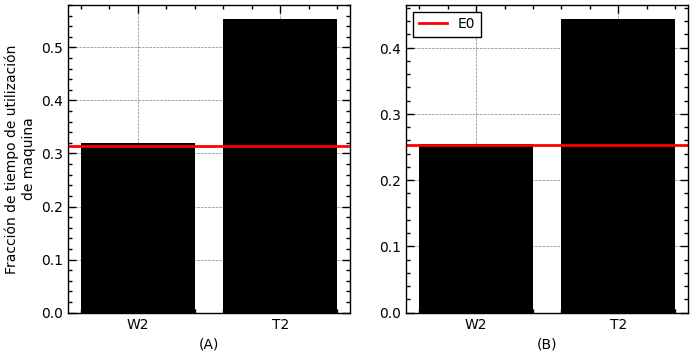
\includegraphics[width=\textwidth]{fig/4_bar_2shift-2techn_comp}
	\end{center}
	\caption{Comparación de el nivel de saturación en tiempo entre: [I] 2 técnicos trabajando simultáneamente, [II] 2 técnicos en distintos turnos.
	(A) Ensayos endurance. (B) Ensayos rolling.}
	\label{fig:4_bar_2shift-2techn_comp}
\end{figure}

\begin{figure}
	\begin{center}
		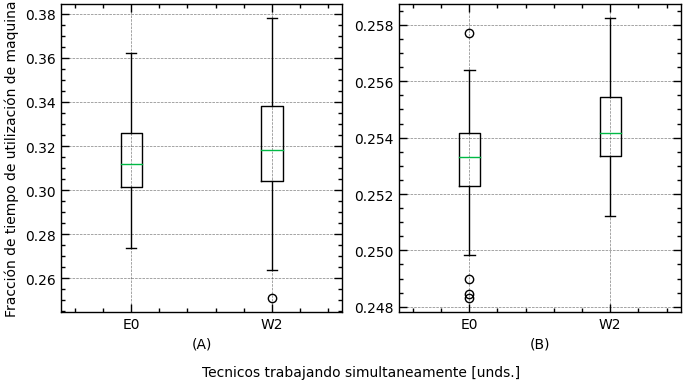
\includegraphics[width=\textwidth]{fig/4_box_techn1-2_comp}
	\end{center}
	\caption{Comparación de el nivel de saturación en tiempo entre 1 técnico y 2 técnicos trabajando simultáneamente.
	(A) Ensayos endurance. (B) Ensayos rolling.}
	\label{fig:4_box_techn1-2_comp}
\end{figure}

Por ultimo, se ha tratado de observar la en el rendimiento de ensayos
que aportaría la instalación de nuevas maquinas para el ensayo endurance.
En la Figura~\ref{fig:4_sctr_indoor}, se observa como añadir maquinas
no aumenta de manera significativa la cantidad de ensayos realizados,
ya que el técnico queda saturado de trabajo con la configuración actual.

Este análisis concluye, que en caso de necesitar capacidad adicional,
se opte por reposicionar a uno de los técnicos
en un turno adicional durante el periodo que sea necesario.
Ya que, es con diferencia la opción mas optima.

\begin{figure}
	\begin{center}
	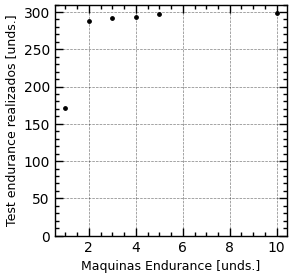
\includegraphics{fig/4_sctr_indoor}
	\end{center}
	\caption{Aumento de los ensayos realizados en función de las maquinas endurance instaladas.}
	\label{fig:4_sctr_indoor}
\end{figure}


\section{METODOLOGÍA}
\section{DESARROLLO}
\section{CONCLUSIONES}

\newpage 

\bibliographystyle{elsarticle-harv}
\bibliography{mybibfile}
\end{document}
